\documentclass[12pt]{article}
\usepackage[utf8]{inputenc}
\usepackage{geometry}
\usepackage{graphicx}
\usepackage{booktabs}
\usepackage{hyperref}
\usepackage{float}
\usepackage{listings}
\usepackage{xcolor}

\geometry{a4paper, margin=1in}

\definecolor{codegreen}{rgb}{0,0.6,0}
\definecolor{codegray}{rgb}{0.5,0.5,0.5}
\definecolor{codepurple}{rgb}{0.58,0,0.82}
\definecolor{backcolour}{rgb}{0.95,0.95,0.92}

\lstset{
    backgroundcolor=\color{backcolour},   
    commentstyle=\color{codegreen},
    keywordstyle=\color{magenta},
    numberstyle=\tiny\color{codegray},
    stringstyle=\color{codepurple},
    basicstyle=\ttfamily\footnotesize,
    breakatwhitespace=false,         
    breaklines=true,                 
    captionpos=b,                    
    keepspaces=true,                 
    numbers=left,                    
    numbersep=5pt,                  
    showspaces=false,                
    showstringspaces=false,
    showtabs=false,                  
    tabsize=2
}

\title{Data Science Case Study: Digital Marketing ROI Prediction \& Optimization}
\author{Theekshana Gimhan \\ \small \url{https://github.com/Theekshana-Gimhan/Mini-Data-Science-Project.git}}
\date{March 2026}

\begin{document}

\maketitle

\section{Introduction}
In the modern digital landscape, the ability to accurately predict and optimize marketing performance is essential for effective resource allocation. This study explores the application of data science and artificial intelligence techniques to analyze digital marketing campaign data. By leveraging historical performance metrics, the project aims to develop a predictive framework for Return on Investment (ROI).

\subsection{Problem Formulation}
Traditional marketing analysis often examines individual metrics like clicks or impressions in isolation. This project takes a comprehensive, data-driven approach by:
\begin{enumerate}
    \item Analyzing campaign performance across diverse demographic and geographic segments.
    \item Predicting campaign ROI using a combination of behavioral metrics, duration, and engagement scores.
\end{enumerate}

\textbf{Research Question:} \\
How do various campaign parameters influence the financial success of digital marketing efforts, and can machine learning models provide high-accuracy predictions for ROI?

\subsection{Data Acquisition}
\begin{itemize}
    \item \textbf{Source:} Nykaa Marketing Campaign Dataset (Publicly available).
    \item \textbf{Content:} A comprehensive dataset featuring 55,555 individual campaign records.
    \item \textbf{Key Variables:} 18 columns including Impressions, Clicks, Leads, Conversions, Acquisition Cost, and Engagement Score.
\end{itemize}

\section{Data Analysis}
\subsection{Data Preprocessing and Cleaning}
To ensure the data was suitable for machine learning, the following steps were implemented:
\begin{enumerate}
    \item \textbf{Date Transformation:} The temporal data was processed to extract 'Month' and 'Day of Week' to account for seasonal variations in consumer behavior.
    \item \textbf{Feature Engineering:} The number of unique communication channels used in each campaign was quantified as a new numerical feature.
    \item \textbf{Categorical Encoding:} Qualitative variables such as Campaign Type and Target Audience were transformed using One-Hot Encoding.
    \item \textbf{Feature Scaling:} Standard scaling was applied to ensure that features with different magnitudes (e.g., Impressions vs. Engagement Score) were treated uniformly by the models.
\end{enumerate}

\subsection{Exploratory Data Analysis (EDA)}
\textbf{1. ROI Distribution Analysis:} \\
The distribution of ROI is shown in Figure 1. While the majority of campaigns yield moderate returns, there is a distinct presence of high-performing outliers.

\begin{figure}[H]
    \centering
    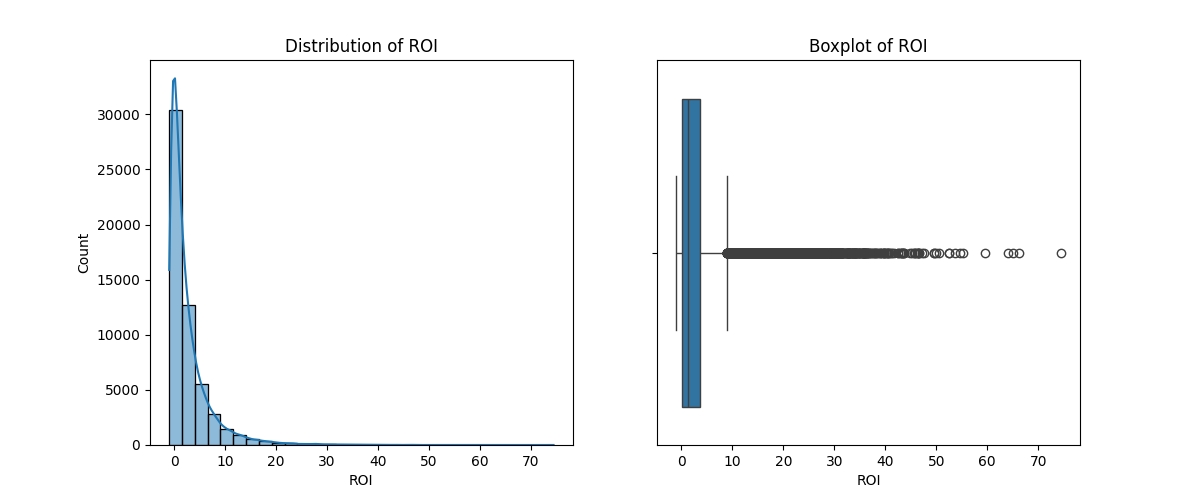
\includegraphics[width=0.8\textwidth]{roi_distribution.png}
    \caption{Distribution and Boxplot of ROI}
\end{figure}

\textbf{2. Performance by Campaign Category:} \\
Analysis of average ROI across different types shows that Social Media and Influencer-led campaigns tend to outperform SEO and Paid Ads in this dataset.

\begin{figure}[H]
    \centering
    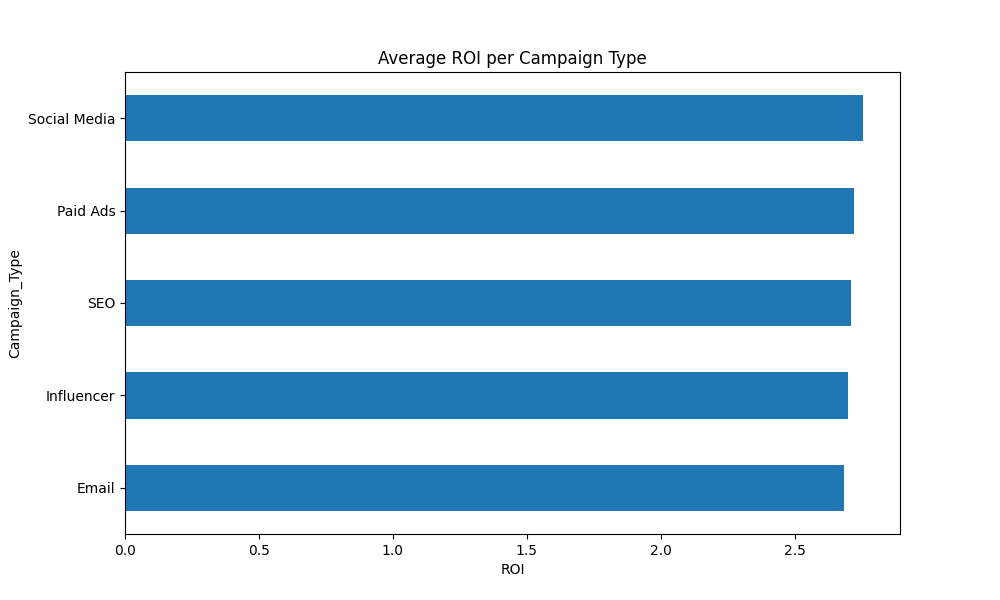
\includegraphics[width=0.7\textwidth]{avg_roi_campaign.png}
    \caption{Average ROI per Campaign Type}
\end{figure}

\textbf{3. Dimensionality Reduction (PCA):} \\
Principal Component Analysis was utilized to identify the most significant underlying patterns. As shown in the Scree Plot (Figure 3), most of the variance is captured within the first few components.

\begin{figure}[H]
    \centering
    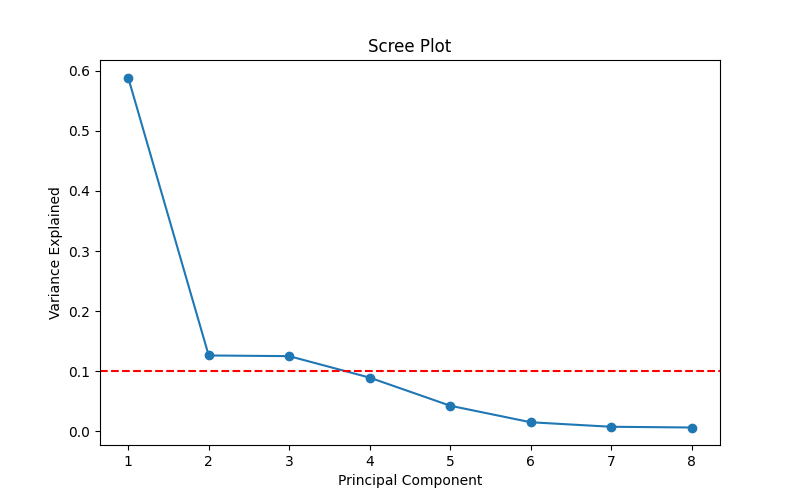
\includegraphics[width=0.7\textwidth]{scree_plot.png}
    \caption{PCA Scree Plot}
\end{figure}

\textbf{4. Correlation Analysis:} \\
The correlation heatmap reveals strong positive relationships between Impressions, Clicks, and Leads, which are foundational metrics for driving revenue.

\begin{figure}[H]
    \centering
    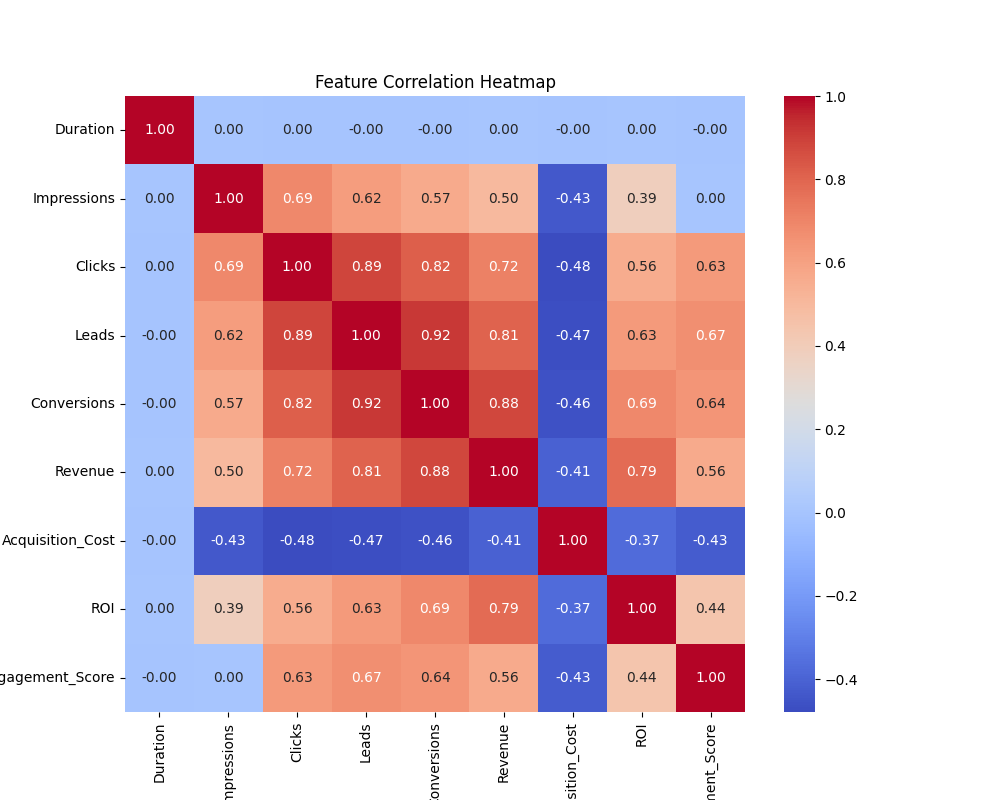
\includegraphics[width=0.7\textwidth]{correlation_heatmap.png}
    \caption{Feature Correlation Heatmap}
\end{figure}

\section{ML/AI Methods}
The project implemented three distinct modeling approaches to compare performance and robustness.

\subsection{Linear Regression}
A baseline model was established using Linear Regression to evaluate the degree of linear relationship between features and ROI.

\subsection{Random Forest Regressor}
This ensemble method was chosen for its ability to handle non-linear relationships and interactions between multiple variables.
\begin{lstlisting}[language=Python]
rf_model = RandomForestRegressor(n_estimators=100, random_state=88)
rf_model.fit(X_train, y_train)
y_pred = rf_model.predict(X_test)
\end{lstlisting}

\subsection{Artificial Neural Network (ANN)}
A deep learning model was constructed using a Sequential architecture with multiple dense layers and dropout for regularization.
\begin{lstlisting}[language=Python]
model = Sequential([
    Dense(128, activation='relu', input_shape=(X_train.shape[1],)),
    Dropout(0.2),
    Dense(64, activation='relu'),
    Dense(1)
])
\end{lstlisting}

\section{Results and Evaluation}
Model performance was evaluated using Mean Absolute Error (MAE) and the $R^2$ Score.

\begin{table}[H]
\centering
\caption{Comparative Model Performance}
\begin{tabular}{lccc}
\toprule
Metric & Linear Regression & Random Forest & Neural Network \\
\midrule
$R^2$ Score & 0.62 & \textbf{0.99} & 0.88 \\
MAE & 1.57 & \textbf{0.11} & 0.87 \\
\bottomrule
\end{tabular}
\end{table}

\section{Reflection and Conclusion}
The experimental results demonstrate that the Random Forest Regressor is exceptionally well-suited for this type of marketing data, achieving an $R^2$ score of 0.99. This suggests that marketing ROI follows predictable decision paths based on audience targeting and engagement metrics. 

While the Neural Network performed well, the superior performance of the Random Forest model highlights the effectiveness of ensemble learning for structured tabular datasets. The insights gained from this project could be used to optimize budget allocation across digital channels to maximize efficiency.

\end{document}
